\documentclass[oneside, a4paper, onecolumn, 11pt]{article}

% Change this: Customize the title, author, advisor, abstract
\newcommand{\thesistitle}[0]{Emotion Recognition in Conversation through Emotion Flow}
\newcommand{\authorname}[0]{Bruno Iorio}

\newcommand{\supervisor}[0]{Gaël Guibon}
\newcommand{\supervisorinstitution}[0]{LIPN - Université Sorbonne Paris Nord}

\newcommand{\abstracttext}[0]{%
  Emotion Recognition in Conversation (ERC) is a very important domain, which has been gaining more attention in recent years, 
  especially within NLP. In the scope of Emotion Recognition, identifying emotions in dialogues plays an essential role. This is because 
  most of the emotional text data collection happens in the context of a conversation between two or more parties (e.g. customer service survey).
  In this paper we discuss the limitation of previous approches to the ERC task, while also evaluating an original approach
  to the same problem using Causal learning, which we identify as the Emotion Flow and attention mechanisms. (initial version)
}

\usepackage[
  left=2cm,top=2.0cm,bottom=2.0cm,right=2cm,
  headheight=17pt, % as per the warning by fancyhdr
  includehead,includefoot,
  heightrounded, % to avoid spurious underfull messages
]{geometry}


\usepackage[T1]{fontenc}
\usepackage{amstext}
\usepackage{amsmath}
\usepackage{amssymb}
\usepackage{url}
\usepackage{graphicx}
\usepackage{wrapfig}
\usepackage{enumerate}
\usepackage{paralist}
\usepackage{xspace}
\usepackage{color}
\usepackage{times}
\usepackage[colorlinks,linkcolor=blue]{hyperref}
\usepackage[colorinlistoftodos,prependcaption,textsize=normal]{todonotes}
\usepackage{pdfpages}
\usepackage{fancyhdr} %% For changing headers and footers


\usepackage{tikz}
\usetikzlibrary{fit,positioning,hobby}
\usetikzlibrary{decorations.text}
\usetikzlibrary{decorations.pathreplacing}


\usepackage{listings}
\usepackage{hyperref}


\usepackage{titling}
\usepackage[nottoc,numbib]{tocbibind}

%% \predate{}
%% \postdate{}
%% \date{}
%% \author{\authorname}


\begin{document}

%\title{\thesistitle}

%\maketitle

% Max 10 lines.
%\noindent \paragraph*{Abstract}
%\abstract

\hspace{0pt}
\vfill

\begin{center}


\includegraphics[width=0.3\textwidth]{img/logo-EP-vertical}

\vspace*{2em}
%
{\large
\textbf{\'Ecole Polytechnique}

\vspace*{1em}
\textit{BACHELOR THESIS IN COMPUTER SCIENCE}


\vspace*{3em}
{\Huge \textbf{\thesistitle}}
\vspace*{3em}



\textit{Author:}

\vspace*{1em}
\authorname{}, \'Ecole Polytechnique

\vspace*{2em}
%
{\textit{Advisor:}}

\vspace*{1em}
\supervisor{}, \supervisorinstitution{}
}

\vspace*{2em}
\textit{Academic year 2024/2025}

\end{center}

\vfill
\hspace{0pt}

\newpage

\vfill
\noindent\textbf{Abstract}\\[1em]
%
\fbox{
\parbox{\textwidth}{
\abstracttext{}
}
}
\vfill


\newpage

% Setting up the header
\pagestyle{fancy}
%\renewcommand{\headrulewidth}{0pt} % Remove line at top
%\renewcommand{\headrulewidth}{0.4pt}% Default \headrulewidth is 0.4pt
\lhead{\authorname}
%\chead{\acronym}
\rhead{\thesistitle}



\newpage
\tableofcontents
\newpage

%\pagenumbering{arabic}

\section{Introduction}  % I am thinking of adding overview on the topic + Related work
\subsection{Background}
Emotions can be understood as the psicological state of an individual, which can be directly influenced by external factors.
In human interactions, they serve as a natural response to these external agents, affecting communication, actions, speech tone, etc.
Emotion Recognition (ER) deals with the problem of detecting emotions in speech, and this comes with the challenge of studying how 
different factors -- such as context -- can shape emotions. Studying ER, therefore, provides us important information about the dynamics 
in human communication.

\begin{center}
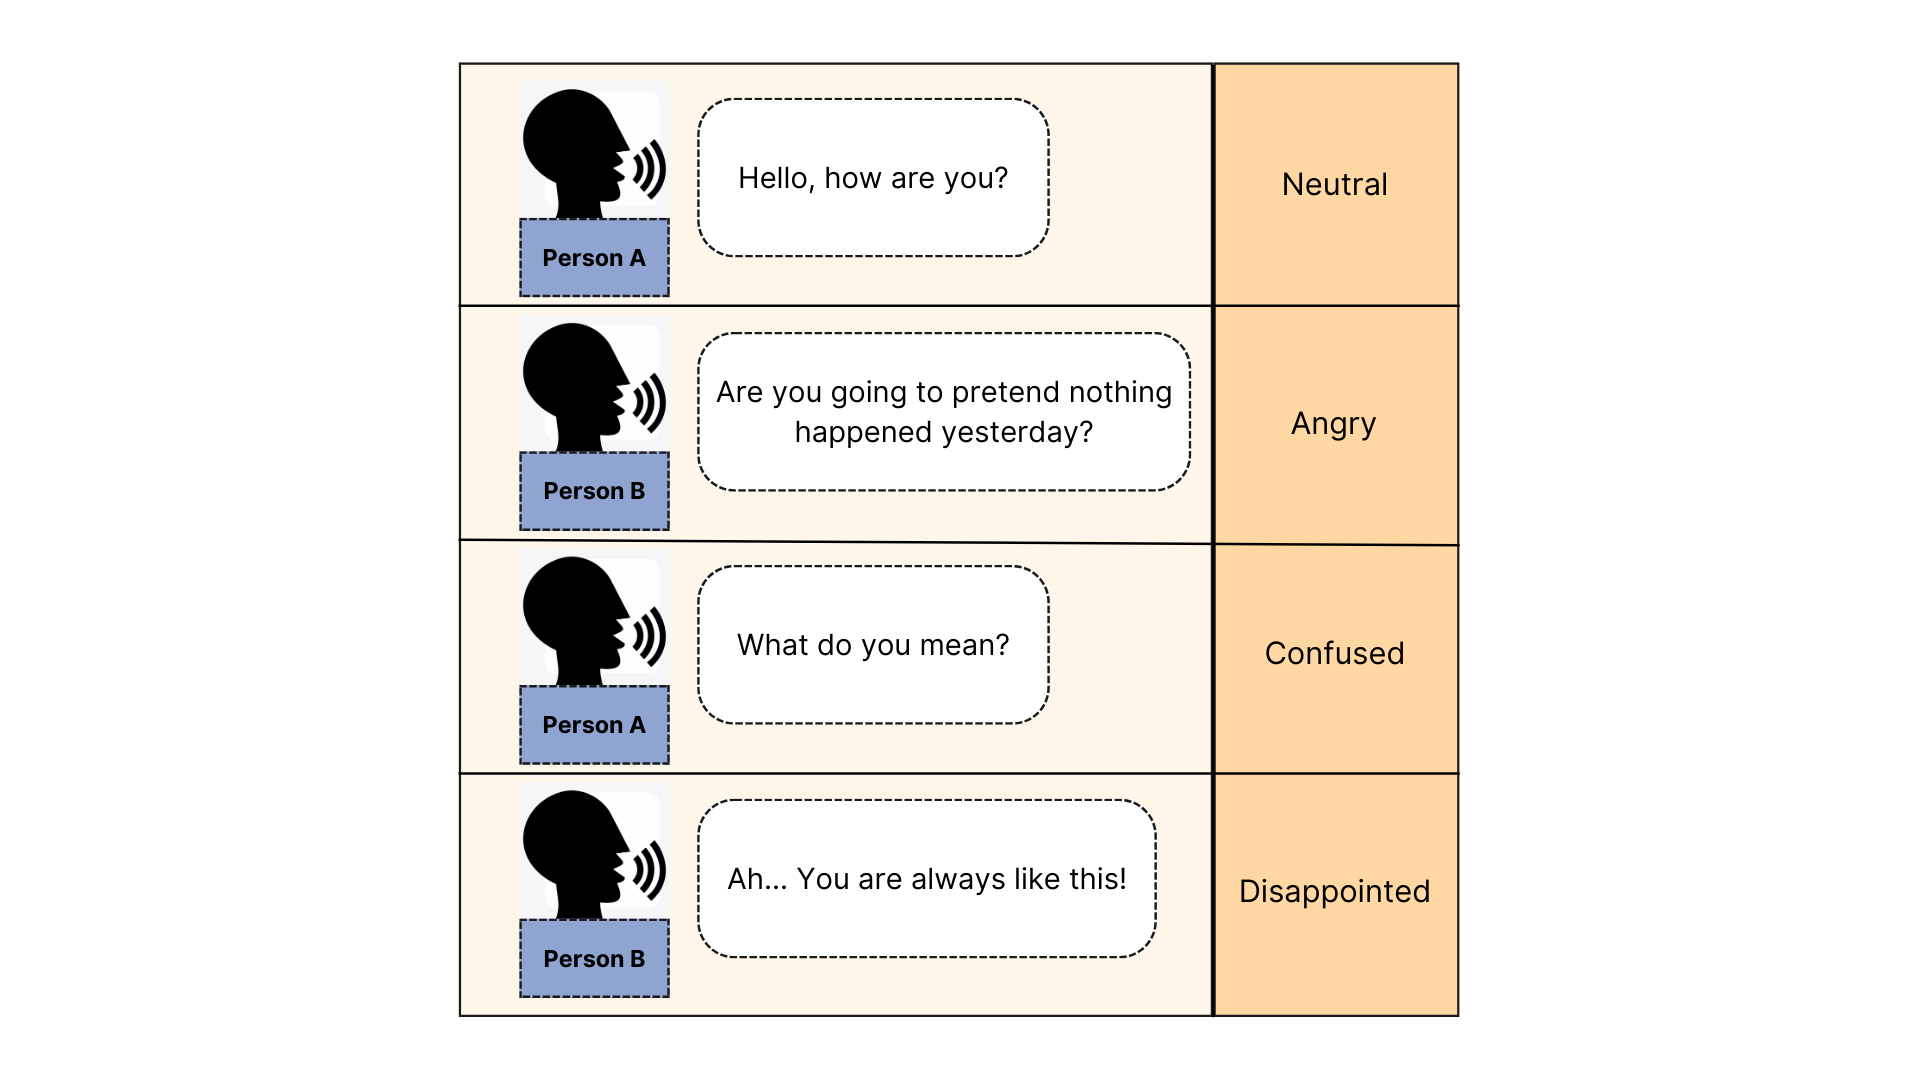
\includegraphics[width=0.8\textwidth]{img/dialogue_example/conversation}
\end{center}

Emotion Recognition in Conversation (ERC) is a growing field within NLP which tackles the task of identifying emotions in conversation. 
The collection of emotional data through conversation provides a realistic, and rich source of information compared to isolated text examples.
Having this information, and utilising it properly has become increasingly important in many different sectors. For instance, companies can 
leverage ERC to measure customer's satisfaction, allowing a better perspective on how to improve their services.

Restricting Emotion Recognition to text has he benefit of allowing us to maintain many important emotional agents, while keeping compact and 
easy-to-process data. However, it eliminates factors that are strongly connected to emotions, such as voice tone, gestures, facial expressions 
etc. This imposes strong limitations on emotion detection task, and limits the extend to which we can study emotions. Also, disambiguating 
emotions becomes severely more complex: emotions that are already very nuanced -- such as joyfulness, hapiness, excitement etc -- become even 
harder to be distinguished, when we surpress multiple emotional factors.

In order to overcome these challanges, many resources were introduced in ERC. Recent research has been strongly focused on understanding the strong and 
weak points of different architectures when applied to this task. DialogueRNN \cite{majumder2019dialoguernnattentivernnemotion}, leverages recursive and 
attention mechanisms, to retrieve a "party state", for each of the parties in the conversation, which is later used to classify each emotion. 
It compares how different recursive modules -- such as LSTMs, and GRUs -- in the same task. Task-Oriented Dialogue \cite{stricker2024unifiedapproachemotiondetection} 
have been integrated with LLMs for ERC, by providing emotion recognition tasks for fine-tunned LLMs. This work, however, overlooks the fact that LLMs
may are trained on many publicly available datasets, possibly including the ones their models were tested on.

\subsection{Task definition}
An important factor influencing emotion is the Emotion Flow (EF), which can be defined as the graph describing the evolution of emotions 
throughout a conversation. It allows us to add an extra depth into the emotion recognition task, and it can address many issues, such as 
emoitonal disambiguating. Researchers believe that emotions have a certain resistance to change over time, a concepted known as Emotional inertia.
It implies that previous emotions have a strong impact on future emotions, which strongly motivates us to study EF. To the best of our knowledge, 
previous research has only studied Emotion Flow in an utterance level, by predicting emotions for each utterance. So, the question whether other 
treatments to emotion prediction could be effective still remains to be answered. More especially, we raise the question whether a word level approach, 
by predicting an emotion for each word in the conversation, could be effective.

In this Project, we aim at evaluating how a word level approach can be combined with the Emotion Flow in the ERC task. Along with this, we also evaluate 
how predicting tokens along with the emotions, in a word-level approach can affect the performance of the models.

\begin{center}
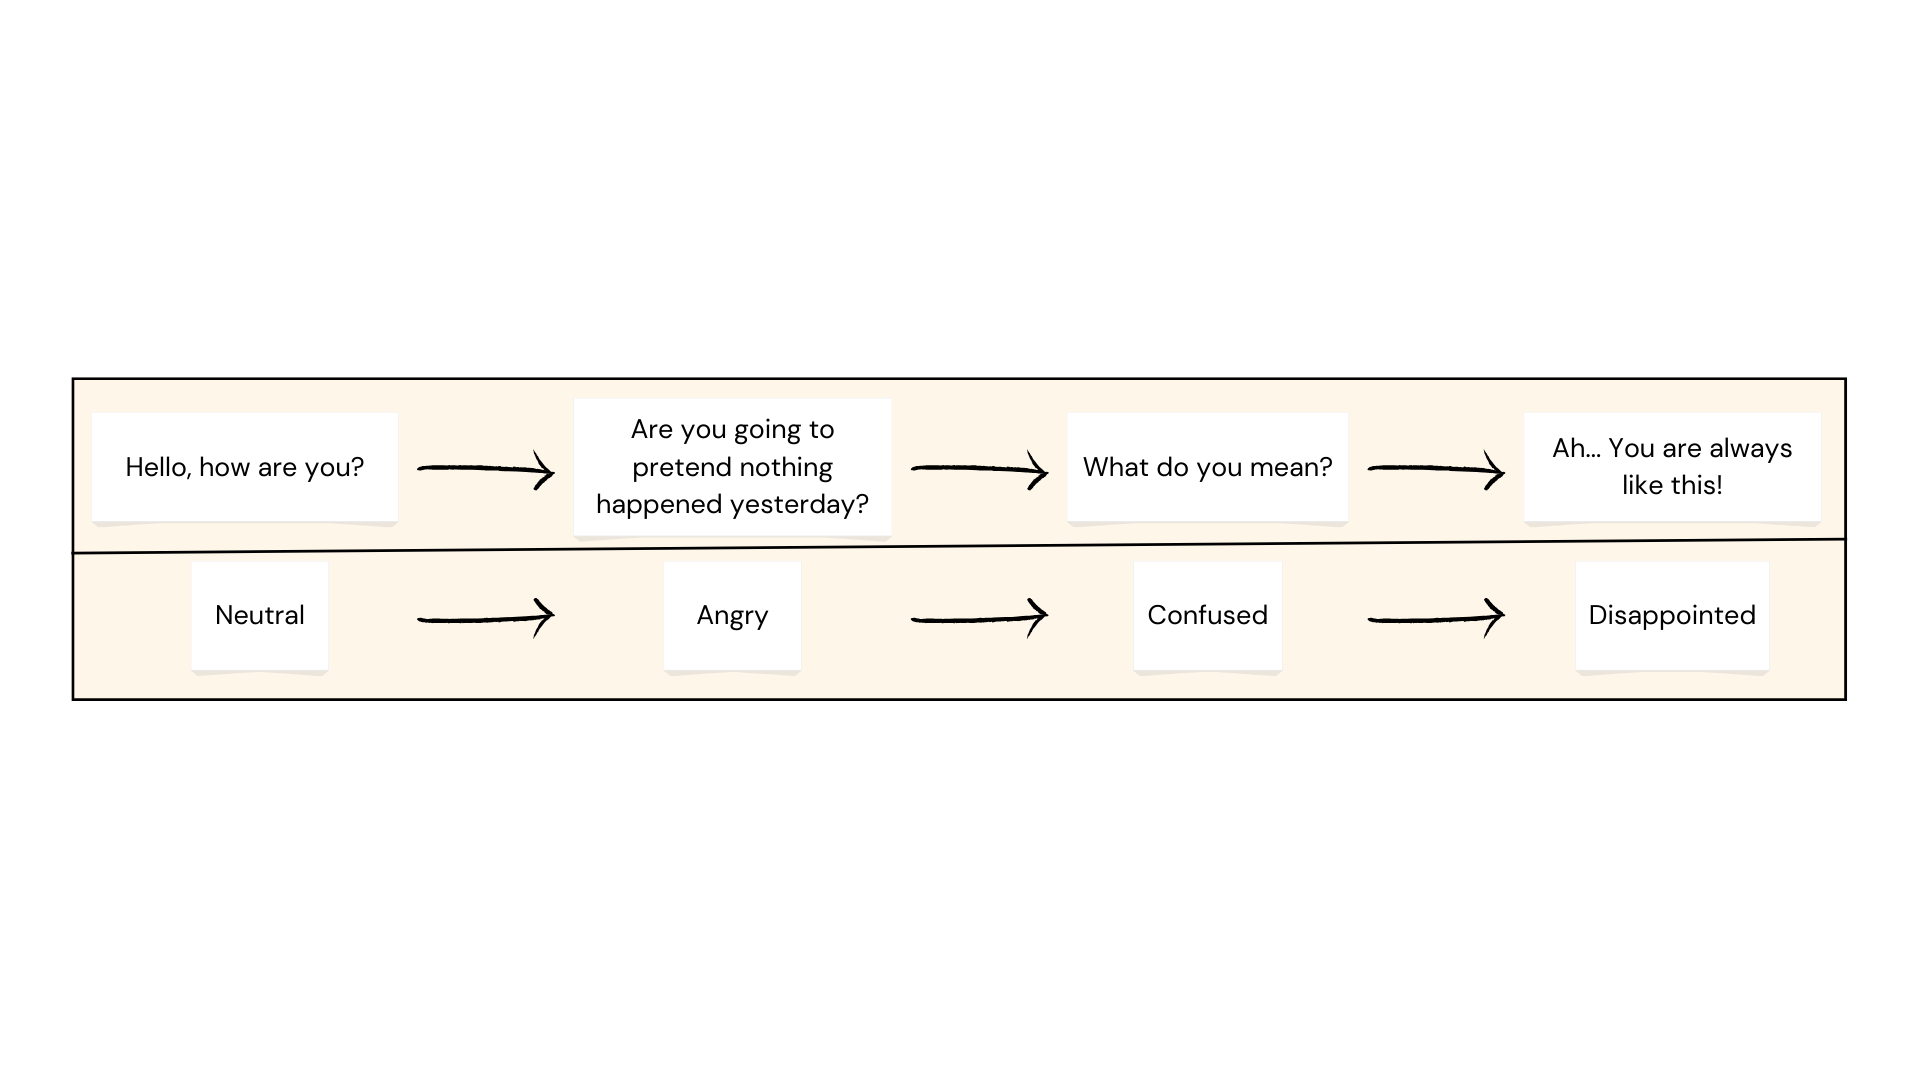
\includegraphics[width=0.8\textwidth]{img/dialogue_example/emotion_flow}
\end{center}

\subsection{Contributions}
\textbf{complete this later}
All the work presented in this report can be found \href{https://github.com/bruno-iorio/thesis-work}{here}.


\section{Related Work} 
Many interesting methods were previously used in ERC. In \cite{LIU2025126924}, it is applied a window transformer - using narrow
2D window masks - to catch short-term inter-utterance relations, used in the task of Causal Emotion Entailment(CEE), e.g. determining
which parts of the text are causing each emotion. This was particularly inspired from MPEG \cite{10252019}, where the emotional information 
is embedded and later on fused with the textual information using an attention layer. This is useful because the CEE is closely related to ERC,
and actually its use can actually improve the effeciency of ERC models \cite{LIU2025126924}. In \cite{wang-etal-2024-emotion}, the model 
also predicts a personality profile vector for each individual participating in the conversation, by using BERT, with a multilayer perceptron.
This is integrated with a fine-grained classification  module, that predicts an emotion for each utterance. In \cite{qin2023bertercfinetuningbertemotion}, they achieve
good performance in the ERC task by applying prompting engeneering techniques, following with a fine-tunned BERT classifier. Comparatively, it 
is a very simple approach to this problem.

Many of the previous works provide us ways of fusing the emotion information with the textual information, while not overcomplexifying the overall 
archtectures of the models. However, they don't address different approaches for the treatment of the Emotion Flow, specially how a word-level approach
would perform.




\section{Datasets used}

Througout this project, we considered the following options of datasets:

\textbf{DailyDialog: } \cite{li2017dailydialogmanuallylabelledmultiturn} Dataset containing 14,118 dialogues representing daily life dialogue situations. Each 
utterance is classified with one of the following emotions: anger, disgust, fear, happiness, sadness, surprise or other(no emotion).

\textbf{MELD: } \cite{poria2019meldmultimodalmultipartydataset} Dataset containing emotion anotation for over 1400 dialogues, and 13000 utterances, which were extract
from the Friends TV show. It classifies each utterance as one of the following emotions: anger, disgust, fear, joy, neutral, sadness or surprise.

\textbf{EmoryNLP: } \cite{zahiri2017emotiondetectiontvtranscripts} 12,606 utterances extracted from the Friends TV show. It classifies each utterance as one of the following
emotions: joyful, peaceful, powerful, scared, mad or sad.

After careful consideration, we decided to mainly focus on the EmoryNLP dataset. The reason for this is that EmoryNLP is considerably more balanced than the other two 
datasets, even though having less content than the DailyDialog dataset. This extra variety is positive, because it allows models to learn better the difference between
emotions.

\textbf{Insert Diagram for DD, MELD, EmoryNLP}

\section{Methodology}


\subsection{Text preprocessing}
We used a classic tokenization approach. For each conversation $C$ in the dataset, we applied the tokenizer for each utternation $utt_k$, getting a list of tokens
$[tok_{1,1},tok_{1,2},\cdots, tok_{1,k_1}]$. After, we proceeded to concanate in order each of the tokenized utterances, getting  $[tok_1,tok_2, \cdots, tok_m]$,
where $m$ is the maximum number of words per conversation, set default to $200$.
  $$
  C = [utt_1, \cdots, utt_n] \to \\
  $$
  $$
  [[tok_{1,1},tok_{1,2},\cdots, tok_{1,k_1}], \cdots , [tok_{n,1},\cdots,tok_{n,k_n}]] \to \\
  $$
  $$
  [tok_1,tok_2, \cdots, tok_m]  \\
$$

\subsection{Emotion preprocessing}
\subsection{Models}

\textbf{Simple Recursive Model:}
\begin{center}
    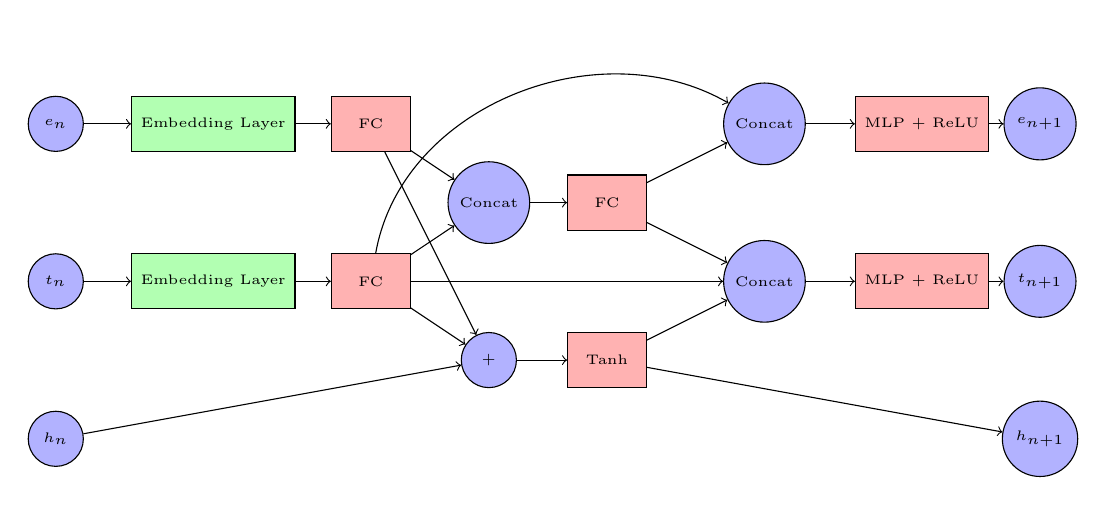
\begin{tikzpicture}[
            neuron/.style={circle, draw, minimum size=0.7cm},
            rect neuron/.style={rectangle, draw, minimum width=1cm, minimum height=0.7cm}, % Rectangular neuron
            input neuron/.style={neuron, fill=blue!30},
            embeddings neuron/.style={rect neuron, fill=green!30},
            mlp neuron/.style={rect neuron, fill=red!30},
            output neuron/.style={neuron, fill=red!30},
            every node/.style={align=center,font=\tiny}
    ]
        % Input Layer
        \node[input neuron] (inp_e) at (0,2) {$e_n$};
        \node[input neuron] (inp_t) at (0,0) {$t_n$};
        \node[input neuron] (inp_h) at (0,-2) {$h_n$};
        
        % Text Processing
        \node[embeddings neuron] (emb_e) at (2,2) {Embedding Layer};
        \node[embeddings neuron] (emb_t) at (2,0) {Embedding Layer};
        
        % Emotion Processing
        \node[mlp neuron] (MLP1_emo) at (4,2) {FC};
        \node[mlp neuron] (MLP1_txt) at (4,0) {FC};

        % Hidden Update
        \node[input neuron, minimum size=0.7cm] (hidden_upd1) at (5.5,-1) {+};
        \node[mlp neuron] (hidden_upd2) at (7,-1) {Tanh};
        
        % Fusion
        \node[input neuron] (concat1) at (5.5,1) {Concat};
        \node[mlp neuron] (mlp_fus) at (7,1) {FC};

        % Final Emotion
        \node[input neuron] (concat2) at (9,2) {Concat};
        \node[mlp neuron] (MLP2_emo) at (11,2) {MLP + ReLU};

        % Final Text
        \node[input neuron] (concat3) at (9,0) {Concat};
        \node[mlp neuron] (MLP2_txt) at (11,0) {MLP + ReLU};

        \node[input neuron] (out_emo) at (12.5,2) {$e_{n+1}$};
        \node[input neuron] (out_txt) at (12.5,0) {$t_{n+1}$};
        \node[input neuron] (out_hidden) at (12.5,-2) {$h_{n+1}$};

        % Arrows
        \draw[->] (inp_t) -- (emb_t);
        \draw[->] (emb_t) -- (MLP1_txt);
        \draw[->] (MLP1_txt) -- (hidden_upd1);
        \draw[->] (MLP1_txt) -- (concat1);
        \draw[->] (MLP1_txt) to[out=80, in=150] (concat2);
        \draw[->] (MLP1_txt) -- (concat3);
        

        \draw[->] (inp_e) -- (emb_e);
        \draw[->] (emb_e) -- (MLP1_emo);
        \draw[->] (MLP1_emo) -- (hidden_upd1);
        \draw[->] (MLP1_emo) -- (concat1);

        \draw[->] (inp_h) -- (hidden_upd1);
        \draw[->] (hidden_upd1) -- (hidden_upd2);
        \draw[->] (hidden_upd2) -- (concat3);
        \draw[->] (hidden_upd2) -- (out_hidden);
        
        \draw[->] (concat1) -- (mlp_fus);
        \draw[->] (mlp_fus) -- (concat2);
        \draw[->] (mlp_fus) -- (concat3);
        
        \draw[->] (concat2) -- (MLP2_emo);
        \draw[->] (MLP2_emo) -- (out_emo);
        
        \draw[->] (concat3) -- (MLP2_txt);
        \draw[->] (MLP2_txt) -- (out_txt);
        

    \end{tikzpicture}
\end{center}


This model integrates contextual information, by using a recursive hidden state. To fuse the textual information with the emotional information,
we use a very simple concatatenation followed by a linear layer.

\begin{itemize}
  \item \textbf{Input token} ($t_n$)
  \item \textbf{Output token }($t_{n+1}$)
  \item \textbf{Input emotion }($e_n$)
  \item \textbf{Output emotion }($e_{n+1}$)
  \item \textbf{n-th Hidden state } ($h_n$)
  \item \textbf{Fusion layer output }($f_n$)
    

\end{itemize}

We first encode the text using pretrained Fasttext embeddings, and we encode the emotions with trainable embeddings.
\begin{align*}
  t_n &\leftarrow \text{Embedding}_{text}(t_n) \\
  e_n &\leftarrow \text{Embedding}_{emotion}(e_n) \\
\end{align*}
Then, we forward both in Fully Connected (FC) layers. and we use it to update the hidden state, by summing them up, and we concatenate them into a fusion layer.

\begin{align*}
  f_n &\leftarrow \text{concat}(FC_1(t_n),FC_2(e_n)) \\
  h_{n+1} &\leftarrow \tanh{FC(t_n + e_n)}\\
\end{align*}

We then finally predict the next token $t_{n+1}$ by concatenating $f_n$, $t_n$, and $h_{n+1}$, and passing them through an Multi-Layer Perceptron (MLP) with ReLU.
To predict the next emotion we concatenate $f_n$ and $t_n$, and then we pass them through a MLP with ReLU
\begin{align*}
  t_{n+1} &\leftarrow ReLU(MLP(\text{concat}(f_n,h_{n+1},t_n))) \\
  e_{n+1} &\leftarrow ReLU(MLP(\text{concat}(f_n,t_n))) \\
\end{align*}



\begin{center}
    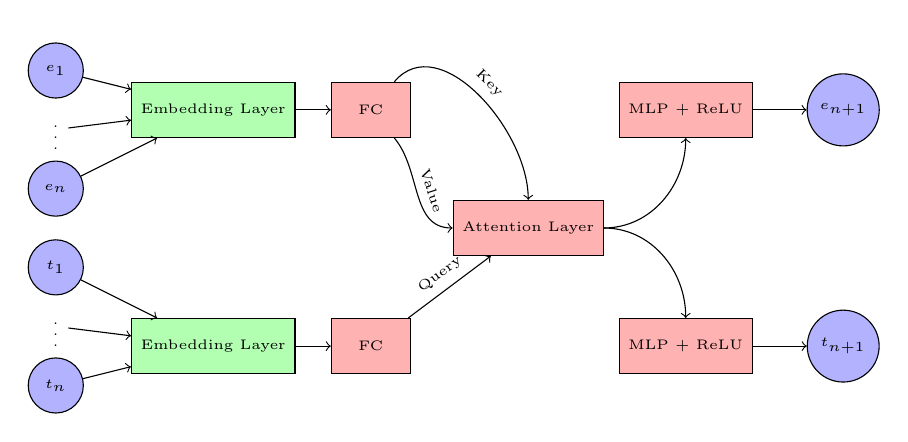
\begin{tikzpicture}[
            neuron/.style={circle, draw, minimum size=0.7cm},
            rect neuron/.style={rectangle, draw, minimum width=1cm, minimum height=0.7cm}, % Rectangular neuron
            input neuron/.style={neuron, fill=blue!30},
            embeddings neuron/.style={rect neuron, fill=green!30},
            mlp neuron/.style={rect neuron, fill=red!30},
            output neuron/.style={neuron, fill=red!30},
            every node/.style={align=center,font=\tiny}
    ]
        % Input Layer
        \node[input neuron] (inp_e1) at (0,2) {$e_1$};
        \node (other_e) at (0, 1.25) {\vdots};
        \node[input neuron] (inp_e2) at (0,0.5) {$e_n$};
        \node[input neuron] (inp_t1) at (0,-0.5) {$t_1$};
        \node (other_t) at (0, -1.25) {\vdots};
        \node[input neuron] (inp_t2) at (0,-2) {$t_n$};
        % Text Processing

        \node[embeddings neuron] (emb_e) at (2,1.5) {Embedding Layer};
        \node[embeddings neuron] (emb_t) at (2,-1.5) {Embedding Layer};

        % Emotion Processing
        \node[mlp neuron] (MLP1_emo) at (4,1.5) {FC};
        \node[mlp neuron] (MLP1_txt) at (4,-1.5) {FC};

        \node[mlp neuron] (attn) at (6,0) {Attention Layer};
        % Final Emotion

        \node[mlp neuron] (MLP2_emo) at (8,1.5) {MLP + ReLU};
        \node[mlp neuron] (MLP2_txt) at (8,-1.5) {MLP + ReLU};

        \node[input neuron] (out_emo) at (10,1.5) {$e_{n+1}$};
        \node[input neuron] (out_txt) at (10,-1.5) {$t_{n+1}$};

        % Arrows
        \draw[->] (inp_t1) -- (emb_t);
        \draw[->] (other_t) -- (emb_t);
        \draw[->] (inp_t2) -- (emb_t);
        \draw[->] (emb_t) -- (MLP1_txt);
        \draw[->] (MLP1_txt) -- (attn) node[pos=0.5,,sloped,above] {Query};

        \draw[->] (inp_e1) -- (emb_e);
        \draw[->] (other_e) -- (emb_e);
        \draw[->] (inp_e2) -- (emb_e);
        \draw[->] (emb_e) -- (MLP1_emo);
        \draw[->] (MLP1_emo) to[out=50,in=90] node[above,sloped] {Key} (attn);
        \draw[->] (MLP1_emo) to[out=-50,in=180] node[above,sloped] {Value} (attn);
        
        \draw[->] (attn) to[out=0,in=-90] (MLP2_emo);
        \draw[->] (attn) to[out=0,in=90] (MLP2_txt);

        \draw[->] (MLP2_emo) -- (out_emo);
        \draw[->] (MLP2_txt) -- (out_txt);

    \end{tikzpicture}
\end{center}





\section{Experimental Protocol}


\section{Results}

\section{Limitation of our approach}

\section{Conclusion}

\section{Perspectives}

\newpage
\nocite{*}
\bibliographystyle{plain}
\bibliography{main}

\newpage
\appendix

\section{Appendix}
\label{sec:appendix}

\end{document}
;
